\chapter{Resultados}\label{chap:resultados}

El penúltimo capítulo se dedica a analizar los resultados obtenidos en la iteración final de las adelantadas en el capítulo \ref{chap:desarrollo} ``Desarrollo''.
Se ahonda en aspectos como las proporciones y composición de los \emph{clusters}, sus centroides, métricas de bondad y en definitiva se explica qué significan estos resultados para este trabajo.

\section{Composición de los clusters}\label{sec:composicionclusters}

Como se adelantaba en la página anterior, más del 80 \% de los equipos de la red se clasifican como comportamientos totalmente normales (subdivididos en dos categorías: normal con muchas conexiones distintas y normal con pocas conexiones).
Algo menos del 10 \% se agrupan en una tercera categoría porque el tráfico de los equipos que la forman es mayoritariamente UDP (lo que implica un comportamiento de características distintas pero no anómalo).
En la cuarta categoría por orden de frecuencia (que supone un 5-10 \% de las instancias) se ha visto otro tipo de tráfico que destaca en unas ocasiones por la larga duración de sus conexiones y en otras ocasiones por el alto número de puertos origen (que indica muchas conexiones).
Y, finalmente, se tiene un último grupo reducido (menos del 1 \%) con casos notablemente anómalos, porque presentan un número de eventos y de puertos destino únicos muy superior al resto.

Esta proporción en la que se han separado los \emph{clusters} es una ventaja, ya que ayuda a centrar la atención en unos pocos casos anómalos que pueden revisarse manualmente.
En la escala del \emph{dataset} obtenido para este trabajo, esa incidencia menor del 1 \% para el grupo muy anómalo supuso siempre menos de 10 casos diarios que pudieron estudiarse individualmente y trasladarse al responsable de la administración de los mismos.

Los demás porcentajes se han mantenido bastante estables a lo largo de los días, así que también será interesante vigilar variaciones respecto a esta estabilidad, como síntoma de un hipotético cambio de tendencia generalizado en el comportamiento de los equipos de la red.

Para permitir examinar los valores específicos que han tomado los centroides en las 8 características más relevantes durante los 7 días, se adjuntan las siguientes tablas de la \ref{tab:dia1} (primer día) a la \ref{tab:dia7} (séptimo día).
Téngase en cuenta que la diferencia de los centroides del primer día respecto al del resto puede explicarse por cuestiones relacionadas con la extracción de los datos,
que incluían sesiones iniciadas varios días atrás, y cómo se han tratado estos datos cortados.
En un procesamiento continuo, este problema no sucedería.

\begin{table}[h]
    \begingroup
    \setlength{\tabcolsep}{2pt} % Default value: 6pt
    \hspace*{-3cm}
    \begin{tabular}{|c|r|r|r|r|r|r|r|r|}
    \hline
    \textbf{Cluster}    & \textbf{dst\_ip} & \textbf{proto} & \textbf{src\_port} & \textbf{dst\_port} & \textbf{max\_prio} & \textbf{count\_events} & \textbf{avg\_duration} & \textbf{stdev\_duration} \\ \hline
    normal, muchas cnxs & 6.02             & 0.00           & 11.60              & 1.66               & 4                  & 37.34                  & 2.81e+04               & 6.25e+04                 \\ \hline
    normal, pocas cnxs  & 2.81             & 0.02           & 3.69               & 1.32               & 5                  & 16.01                  & 6.69e+04               & 3.46e+04                 \\ \hline
    udp                 & 14.37            & 0.91           & 30.72              & 2.09               & 4.19               & 93.90                  & 8.60e+04               & 2.66e+05                 \\ \hline
    cnxs largas         & 7.70             & 0.06           & 12.92              & 2.25               & 4.19               & 1595.12                & 7.2e+06                & 1.40e+07                 \\ \hline
    anom(2)             & 24.65            & 0.49           & 2191               & 2                  & 4.51               & 86121.10               & 8.51e+05               & 3.71e+06                 \\ \hline
    \end{tabular}
    \endgroup
\caption{Valores de los centroides en el día 1}
\label{tab:dia1}
\end{table}

\begin{table}[h]
    \begingroup
    \setlength{\tabcolsep}{2pt} % Default value: 6pt
    \hspace*{-3cm}
    \begin{tabular}{|c|r|r|r|r|r|r|r|r|}
    \hline
    \textbf{Cluster}    & \textbf{dst\_ip} & \textbf{proto} & \textbf{src\_port} & \textbf{dst\_port} & \textbf{max\_prio} & \textbf{count\_events} & \textbf{avg\_duration} & \textbf{stdev\_duration} \\ \hline
    normal, muchas cnxs & 43.84            & 0.04           & 112.67             & 2.04               & 4                  & 296.99                 & 14157.92               & 54004.72                 \\ \hline
    normal, pocas cnxs  & 5.11             & 0.03           & 9.84               & 1.44               & 5                  & 20.30                  & 19812.79               & 20215.99                 \\ \hline
    udp                 & 43.60            & 1.72           & 137.24             & 4.11               & 4.16               & 359.39                 & 65984.58               & 187667.52                \\ \hline
    muchas dst\_ip      & 97.34            & 0.16           & 492.50             & 2.23               & 4                  & 1239.55                & 10575.59               & 66178.72                 \\ \hline
    anom(16)            & 68.50            & 0.31           & 7324.59            & 2.18               & 4.05               & 38265.85               & 4469.58                & 99635.59                 \\ \hline
    \end{tabular}
    \endgroup
\caption{Valores de los centroides en el día 2}
\label{tab:dia2}
\end{table}

\begin{table}[h]
    \begingroup
    \setlength{\tabcolsep}{2pt} % Default value: 6pt
    \hspace*{-3cm}
    \begin{tabular}{|c|r|r|r|r|r|r|r|r|}
    \hline
    \textbf{Clusters}   & \textbf{dst\_ip} & \textbf{proto} & \textbf{src\_port} & \textbf{dst\_port} & \textbf{max\_prio} & \textbf{count\_events} & \textbf{avg\_duration} & \textbf{stdev\_duration} \\ \hline
    normal, muchas cnxs & 58.61            & 0.07           & 257.97             & 2.06               & 4                  & 697.03                 & 34366.40               & 74.43                    \\ \hline
    normal, pocas cnxs  & 4.80             & 0.04           & 9.98               & 1.41               & 5                  & 18.16                  & 7914.26                & 1.78                     \\ \hline
    udp                 & 52.93            & 1.64           & 171.56             & 3.87               & 4.11               & 400.45                 & 65689.04               & 44.95                    \\ \hline
    cnxs largas         & 33.25            & 0.21           & 86.52              & 2.13               & 4.38               & 2015.05                & 722651.46              & 23.28                    \\ \hline
    anom(2)             & 46.50            & 0.50           & 15709.50           & 3                  & 4.50               & 68211.50               & 1                      & 21119.50                 \\ \hline
    \end{tabular}
    \endgroup
\caption{Valores de los centroides en el día 3}
\label{tab:dia3}
\end{table}

\begin{table}[h]
    \begingroup
    \setlength{\tabcolsep}{2pt} % Default value: 6pt
    \hspace*{-3cm}
    \begin{tabular}{|c|r|r|r|r|r|r|r|r|}
    \hline
    \textbf{Cluster}    & \textbf{dst\_ip} & \textbf{proto} & \textbf{src\_port} & \textbf{dst\_port} & \textbf{max\_prio} & \textbf{count\_events} & \textbf{avg\_duration} & \textbf{stdev\_duration} \\ \hline
    normal, muchas cnxs & 57.97            & 0.28           & 253.07             & 2.13               & 4                  & 679.49                 & 10235.43               & 36196.79                 \\ \hline
    normal, pocas cnxs  & 6.02             & 0.10           & 13.55              & 1.44               & 4.99               & 23.83                  & 7345.21                & 9476.48                  \\ \hline
    udp                 & 7.14             & 1.39           & 130.93             & 10.94              & 4.19               & 264.87                 & 20494.34               & 75272.26                 \\ \hline
    cnxs largas         & 40.46            & 0.36           & 114.77             & 2.30               & 4.26               & 489.55                 & 249823.38              & 617650.08                \\ \hline
    anom(1)             & 45               & 2              & 16152              & 4                  & 4                  & 94864                  & 10                     & 1164                     \\ \hline
    \end{tabular}
    \endgroup
\caption{Valores de los centroides en el día 4}
\label{tab:dia4}
\end{table}

\begin{table}[h!]
    \begingroup
    \setlength{\tabcolsep}{2pt} % Default value: 6pt
    \hspace*{-3cm}
    \begin{tabular}{|c|r|r|r|r|r|r|r|r|}
    \hline
    \textbf{Cluster}    & \textbf{dst\_ip} & \textbf{proto} & \textbf{src\_port} & \textbf{dst\_port} & \textbf{max\_prio} & \textbf{count\_events} & \textbf{avg\_duration} & \textbf{stdev\_duration} \\ \hline
    normal, muchas cnxs & 56.84            & 0.33           & 202.58             & 2.17               & 4                  & 523.68                 & 1.02e+04               & 32559.60                 \\ \hline
    normal, pocas cnxs  & 6.21             & 0.08           & 12.88              & 1.50               & 5                  & 21.53                  & 8.96e+03               & 7923.57                  \\ \hline
    udp                 & 26.92            & 0.81           & 107.49             & 5.37               & 4.23               & 408.55                 & 1.01e+05               & 365880.91                \\ \hline
    muchos src\_ports   & 64.25            & 0.01           & 7209.30            & 2                  & 4.13               & 26836.11               & 6.43e+02               & 7962.58                  \\ \hline
    anom(5)             & 1.20             & 0              & 1.20               & 1.01               & 5                  & 141.85                 & 1.92e+06               & 338833.03                \\ \hline
    \end{tabular}
    \endgroup
\caption{Valores de los centroides en el día 5}
\label{tab:dia5}
\end{table}

\begin{table}[h!]
    \begingroup
    \setlength{\tabcolsep}{2pt} % Default value: 6pt
    \hspace*{-3cm}
    \begin{tabular}{|c|r|r|r|r|r|r|r|r|}
    \hline
    \textbf{Cluster}    & \textbf{dst\_ip} & \textbf{proto} & \textbf{src\_port} & \textbf{dst\_port} & \textbf{max\_prio} & \textbf{count\_events} & \textbf{avg\_duration} & \textbf{stdev\_duration} \\ \hline
    normal, muchas cnxs & 55.42            & 0.01           & 227.65             & 2.10               & 3.99               & 610.90                 & 22825.61               & 97734.84                 \\ \hline
    normal, pocas cnxs  & 6.30             & 0.02           & 13.40              & 1.48               & 5                  & 22.57                  & 17373.38               & 15749.55                 \\ \hline
    udp                 & 53.53            & 1.36           & 169.91             & 2.48               & 4.02               & 497.80                 & 18522.75               & 70955.22                 \\ \hline
    cnxs largas         & 5.78             & 1.38           & 115.85             & 11.09              & 4.20               & 256.49                 & 24985.20               & 92374.05                 \\ \hline
    anom(19)            & 75.75            & 0.06           & 7933.31            & 2.18               & 4.06               & 30504.37               & 856                    & 25463                    \\ \hline
    \end{tabular}
    \endgroup
\caption{Valores de los centroides en el día 6}
\label{tab:dia6}
\end{table}

\begin{table}[h!]
    \begingroup
    \setlength{\tabcolsep}{2pt} % Default value: 6pt
    \hspace*{-3cm}
    \begin{tabular}{|c|r|r|r|r|r|r|r|r|}
    \hline
    \textbf{Cluster}    & \textbf{dst\_ip} & \textbf{proto} & \textbf{src\_port} & \textbf{dst\_port} & \textbf{max\_prio} & \textbf{count\_events} & \textbf{avg\_duration} & \textbf{stdev\_duration} \\ \hline
    normal, muchas cnxs & 54.51            & 0.04           & 257.24             & 2.02               & 4                  & 660.99                 & 9426.71                & 33187.10                 \\ \hline
    normal, pocas cnxs  & 5.54             & 0.01           & 17.40              & 1.38               & 4.99               & 34.45                  & 8385.74                & 9746.59                  \\ \hline
    udp                 & 50.07            & 1.60           & 234.74             & 2.48               & 4.11               & 602.45                 & 16391.64               & 57167.76                 \\ \hline
    cnxs largas         & 6.15             & 0.66           & 65.48              & 5.41               & 4.48               & 367.28                 & 503875.35              & 735594.61                \\ \hline
    anom(28)            & 68.48            & 0.07           & 8785.88            & 2.07               & 4.03               & 35278.18               & 771.92                 & 6427.07                  \\ \hline
    \end{tabular}
    \endgroup
\caption{Valores de los centroides en el día 7}
\label{tab:dia7}
\end{table}

\section{Calidad del resultado}\label{sec:calidadresultado}

Existen diversas métricas de bondad para conocer de forma objetiva la calidad del \emph{clustering}, aparte de lo útil que resulte para la aplicación en cuestión.
Aquí se comentan algunas de ellas.

Se mencionaba antes que el ratio de sumas de cuadrados, indicador del equilibrio entre cohesión interna y separación entre \emph{clusters}, era una de las métricas de bondad vigiladas durante los ensayos.
En el resultado final, con agregación diaria, este ratio se incrementó hasta alcanzar el 0.4133 en el peor día y 0.5064 en el mejor.
Esto es señal de que se ha logrado una separación en grupos equilibrada.

Otro indicador estudiado ha sido el coeficiente de silueta, un valor diseñado en \cite{Rousseeuw_1987} y ampliamente usado para interpretar y validar la coherencia del \emph{clustering}.
En el artículo donde se especificó también se propuso una representación gráfica que simboliza lo bien que se ha clasificado cada instancia.

El coeficiente de silueta medio calculado para el resultado final es de 0.476, un índice perfectamente aceptable.
En la figura \ref{fig:silhouette} se observa cuánta similitud guarda una instancia con su \emph{cluster} en comparación con el resto de \emph{clusters}.
Los posibles valores de este índice van de -1 a +1, por lo que se aprecia en la gráfica que la disposición de los \emph{clusters} es apropiada.
En especial, las instancias del \emph{cluster} etiquetado con el 2 (el de las anomalías, más difícil de ver en la figura porque tiene muchas menos instancias) están claramente separadas del resto.

\begin{figure}[h]
    \centering
    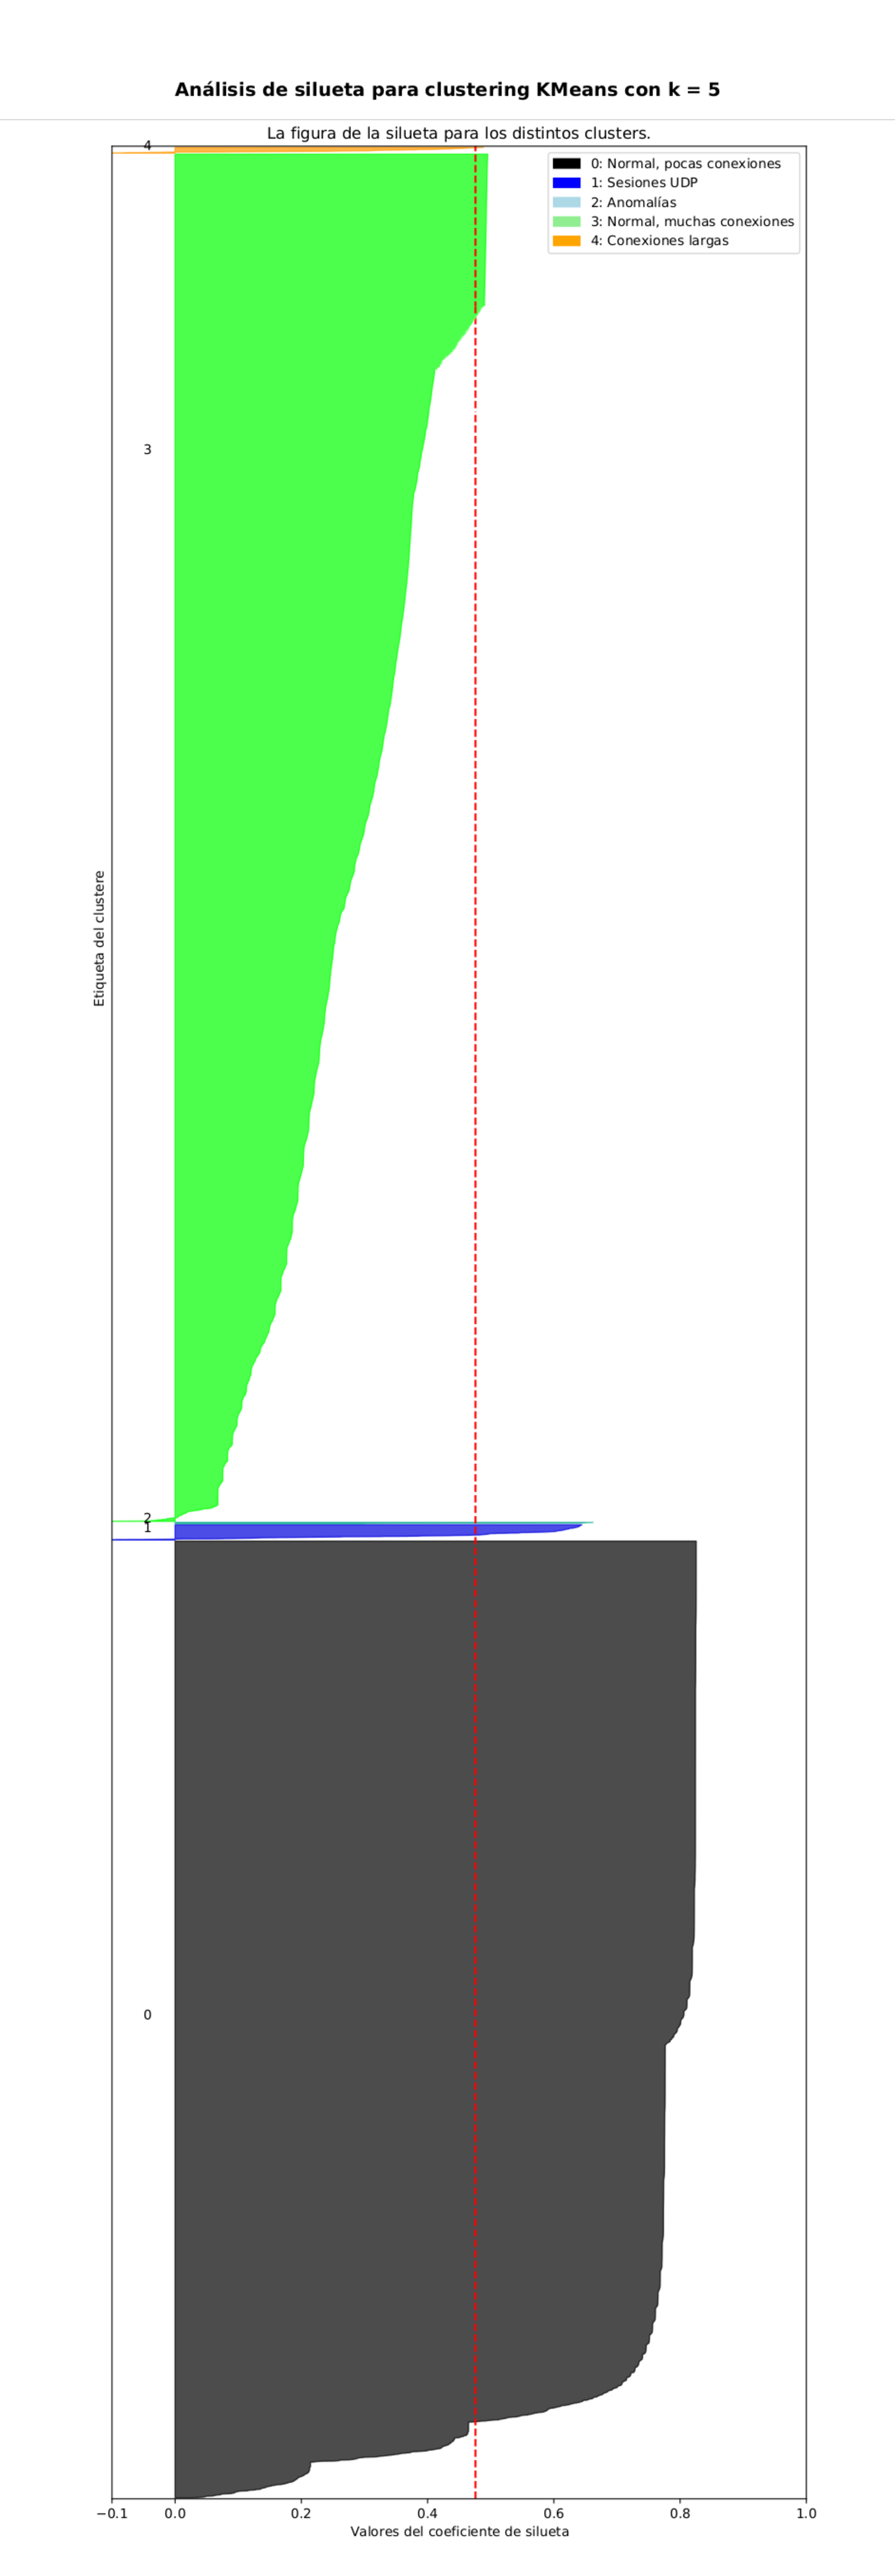
\includegraphics[height=\textheight]{../figures/silhouette_cropped.pdf}
    \caption{Representación gráfica del análisis de silueta para los \emph{clusters} obtenidos con $k=5$}
    \label{fig:silhouette}
\end{figure}
